\documentclass[12pt]{article}

% packages
\usepackage[english]{babel}
\usepackage[utf8]{inputenc}
\usepackage{amsmath}

\usepackage{tocloft}
\usepackage[title,titletoc]{appendix}
\usepackage{fancyhdr}
\usepackage{float}
\usepackage{graphicx, wrapfig, subcaption, setspace, booktabs}

\usepackage{fancyvrb}  % for code verbatim and console outputs
\usepackage[dvipsnames]{xcolor}

\usepackage{xpatch}

\makeatletter
\xpatchcmd{\@chapter}{\addcontentsline{toc}{chapter}{\protect\numberline{\thechapter}#1}}{%
                      \addcontentsline{toc}{chapter}{\protect\numberline{}#1}}{\typeout{Success}}{\typeout{Failed!}}
\makeatother

% margins and widths
\addtolength{\oddsidemargin}{-0.75in}
\addtolength{\evensidemargin}{-0.75in}
\addtolength{\textwidth}{1.75in}

\addtolength{\topmargin}{-0.75in}
\addtolength{\textheight}{1.75in}

% headers / footers
\pagestyle{fancy}
\fancyhf{}
\lhead{\fancyplain{}{8086 Board Design Project}}
\cfoot{\fancyplain{}{--- \thepage \ ---}}

% table of content
\setcounter{tocdepth}{3}
\setcounter{secnumdepth}{3}
\cftsetindents{section}{0.1in}{0.5in}
\cftsetindents{subsection}{0.65in}{0.5in}
\cftsetindents{subsubsection}{0.8in}{0.5in}

% custom commands
% replace '\\' with `\n' to get rid of tab in new paragraphs
\newcommand{\n}{\newline\newline}

\definecolor{dkgreen}{rgb}{0,0.6,0}
\definecolor{gray}{rgb}{0.5,0.5,0.5}
\definecolor{mauve}{rgb}{0.58,0,0.82}
\definecolor{black}{rgb}{0,0,0}

% redefine \VerbatimInput
\RecustomVerbatimCommand{\VerbatimInput}{VerbatimInput}%
{fontsize=\small}

% content
\begin{document}

    \begin{titlepage}

    \newcommand{\HRule}{\rule{\linewidth}{0.5mm}}
    \center

    \HRule \\[0.5cm]
    {\huge \bfseries 8086 Microprocessor Design Project}\\[0.4cm]
    \HRule \\[1.5cm]

    \large{CMPE 310\linebreak Sabbir Ahmed}\\[3cm]

    {\large \today}\\[2cm]

    \begin{figure}[h]
        \begin{center}
            
\includegraphics[width=0.3\textwidth]{figures/uni_logo.jpg}
            \label{fig:uni_logo}
        \end{center}
    \end{figure}

    \vfill % fill the rest of the page with whitespace

\end{titlepage}

    \tableofcontents
    \newpage
\section{Introduction}
This document provides detailed instructions to develop an 8086 microprocessor board using Cadence\textregistered \ OrCAD\textregistered \ Capture software. Included are the schematics of individual IC components and their description. Details of the ICs include decoding, programming specifications, and descriptions of IC pinouts.

    \subsection{Purpose}
    As per the project description, this document is to serve as the only documentation of the operational and functional specifications of the Intel 8086. The documentation is to be thorough and concise to provide information to design a similar board.

    \subsection{Scope and Organization of Document}
    This report 

    \newpage
\section{8086 Microprocessor}
The 8086 microprocessor is an enhanced version of the 8085 microprocessor developed by Intel in 1978. It is a 16-bit microprocessor, with 20 address lines and 16 data lines to provide up to 1 MB of physical memory. 

    \begin{figure}[h]
        \begin{center}
            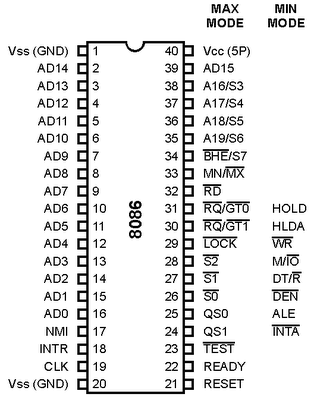
\includegraphics[width=0.35\textwidth]{figures/01_8086.png}
            \caption{8086 Microprocessor} \label{fig:8086}
        \end{center}
    \end{figure}

    \subsection{Features}
    The 8086 microprocessor is known for its significant advancements since its predecessors. The most prominent features include, but are not limited to:

        \begin{itemize}

            \item 6 bytes of cache memory for faster processing

            \item Pipelining stages: Fetch Stage and Execute Stage

            \item Instruction queue

            \item 256 vectored interrupts

            \item Maximum and minimum modes of operation, suitable for multiple and single processors respectively

        \end{itemize}

        \begin{figure}[h]
            \begin{center}
                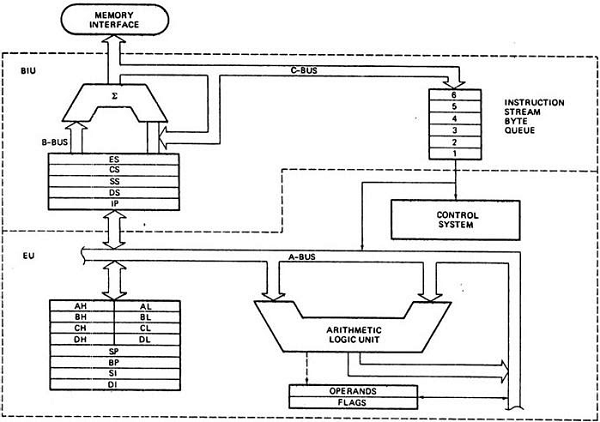
\includegraphics[width=0.65\textwidth]{figures/02_8086_architecture.jpg}
                \caption{Architecture of 8086} \label{fig:8086_architecture}
            \end{center}
        \end{figure}

    \subsection{Address and Data Buses}
    The 8086 CPU has a unidirectional address bus with 20 address lines and a bidirectional data bus with 16 data lines. \cite{buses} The address bus is used to select the desired memory or I/O device by generating a unique address which corresponds to the memory location or the location of I/O device of the system. The data bus is used to transfer data between the CPU and memory and the CPU and I/O devices.\\

    The address bus is denoted as $A_{19}-A_{0}$ (20 lines) and the data bus $D_{15}-D_{0}$ (16 lines). The peripheral devices implemented with the 8086 in this document however consist of 8-bit data bus architectures. The data bus would therefore be multiplexed and more commonly denoted as $D_{7}-D_{0}$ (8 lines).

    \subsection{Control Bus}
    The control bus of 8086 carries control signals which are used to specify the memory and I/O devices. \cite{buses} The bus is bidirectional and assists the CPU in synchronizing control signals to internal devices and external components. It is comprised of interrupt lines, byte enable lines, read/write signals and status lines.

    \subsection{Pinouts}
    Refer to Appendix \ref{appendix:pinouts} for the pinouts of the chip.

    \section{Decoding}

    \subsection{Programming Logic Device - 16L8}

    \subsection{Programming the PLD}

    \newpage
\section{Clock Generator - 8284A}
The 8184A Clock Generator is an ancillary component to the 8086. This system clock is used to synchronize both internal and external operations using an external oscillator. The device is also used for READY and RESET synchronizations and TTL-level peripheral clock signal generation.

        \begin{figure}[h]
            \begin{center}
                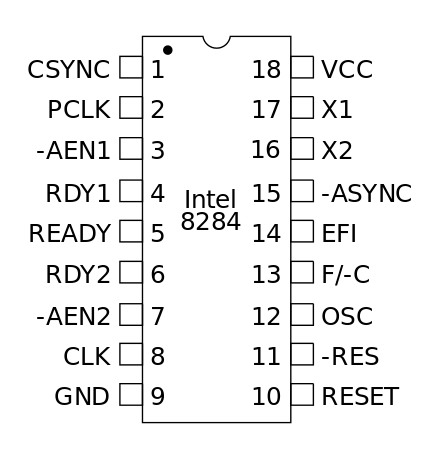
\includegraphics[width=0.4\textwidth]{figures/8284a.png}
                \caption{8284A Clock Generator} \label{fig:8284a}
            \end{center}
        \end{figure}

    \subsection{Clock Speed}
    The 8086 internal clock has a frequency of 5 MHz ($\frac{1}{3}$ of CLK). The external crystal typically oscillates at 15 MHz.

    \subsection{RESET Operation}
    Correct reset timing requires that the RESET input to the 8086 becomes a logic 1 in 4 clock cycles and remain high for at least 50 $\mu S$. The reset switch is implemented in a RC circuit with typical resistance of $100 \ k\Omega$ and $10 \ \mu F$.

    \subsection{Pinouts}
    Refer to Appendix \ref{appendix:pinouts} for the pinouts of the chip.

    \section{Memory Architecture}
The board implemented in this document consists of 128 kB of SRAM and 256 kB of CMOS flash memory.

    \subsection{Static Random Access Memory - CY7C199}
    Static RAM, or SRAM, is a type of volatile memory where bits are stored as long as power is supplied. They are ideal for cache memory because of their fast access times as low as 10 ns. CY7C199 SRAM chips are used to implement the SRAM on this system.

    \subsection{Addressing}
    The SRAM implemented in the system is composed of 32k $\times$ 8 CY7C199 SRAM chips decoded into two banks, with the lowest address at 0x00000.

    \subsection{CMOS Flash Memory - 28F010}
    Flash memory, or electrically erasable programmable ROM (EEPROM), is a type of non-volatile memory which maintains its state even after loss of power. Writing to this memory is much slower than a normal RAM, and it is used to store setup information. 28F010 CMOS chips are used to implement the flash memory on this system.

    \subsection{Addressing Flash Memory}
    The flash memory implemented in the system is composed of 128k $\times$ 8 28F010 CMOS chips decoded into two banks, with the highest address at 0xFFFFF.

    \subsection{Pinouts}
    Refer to Appendix \ref{appendix:pinouts} for the pinouts of the chips.

    \section{Programmable Peripheral Interface}
The 82C55A is a popular interfacing component that can interface any TTL-compatible I/O device to the microprocessor. The chip is used to interface the keyboard and the LCD controller in the system.

    \subsection{Addressing}
    The 3 82C55 chips are decoded at the following port addresses respectively:

        \begin{itemize}

            \item 0x000F (control register), 0x000D, 0x000B, 0x0009

            \item 0x000E (control register), 0x000C, 0x000A, 0x0008

            \item 0x0007 (control register), 0x0005, 0x0003, 0x0001

        \end{itemize}

    \subsection{Assembly Implementation and Programming of the 82C55A}

    \section{Programmable Keyboard/Display Interface - 8279}
16 push button switches connected as four rows and four columns, 2 push button switches connected to the control and shift inputs as well as the reset switch connected to the IR0 pin of the 8259 interrupt controller and NMI keys are arranged as the 5$\times$4 keyboard matrix into the 8279 keyboard controller for the system.

    \subsection{Addressing}
    The 8279 keyboard controller is decoded at 0x00F2 (command) and 0x00F0 (data).

    \subsection{Assembly Implementation}
    The implementation of the keyboard controller is provided in Section \ref{sec:keybrd_asm} of Appendix \ref{appendix:code}.

    \section{Programmable Interval Timer - 8254}
An 8254 programmable interval timer chip is integrated into the system. The component is required to solve the common timing control problems in the microprocessor. The chip also facilitates in other aspects of the system, such as accurate time delays, real time clocks, event counters, square wave generation, etc. The 8254 has 3 independent 16-bit programmable counters, each capable of counting in binary or binary coded decimal (BCD) with a maximum frequency of 1 MHz.\n
All the counter gate, clock and output pins are connected to headers for external access, with the exception of Counter 2 output connected to IR1 of the 8259 interrupt controller.

    \subsection{Addressing}
    The 8254 is decoded at 0xFFEE (command register), 0xFFEC, 0xFFEA and 0xFFE8.

    \subsection{Programming}
    Each of the counters is individually programmed by writing a control word followed by the initial count. The control word is used to select the counter, mode of operation, binary or binary coded decimal counter, and the type of operation.

    \subsection{Assembly Implementation}
    A code segment of interfacing with the interval timer is provided in Section \ref{sec:pit_asm} of Appendix \ref{appendix:code}.

    \section{Universal Asynchronous Receiver/Transmitter  - 16550}
The UART is a programmable communications interface designed to connect to virtually any type of serial interface. The 16550 includes a programmable baud rate generator and separate FIFO buffers for input and output data, and is capable of transmitting and receiving data without a clock or timing signal.

    \subsection{Addressing the 16550}
    The 16550 is decoded in the high bank at odd port addresses from 0x00EF to 0x00E1.

    \subsection{Assembly Implementation}
    A code segment of interfacing with the interval timer is provided in Section \ref{sec:uart_asm} of Appendix \ref{appendix:code}.

    \subsection{MAX-235 and D-SUB-9}
    The MAX-235 is used as an intermediate step between the board and any outside connections requiring 12 V signals. The chip acts in a scaling capacity, either increasing or decreasing the signal voltage from 5 V to 12 V, or vice versa.\n
    The D-SUB-9 is a simple connection adapter for the inputs and outputs.

    \section{Interrupt Controller - 8259}

    \subsection{Implementing a Master Interrupt Controller}

    \subsection{Addressing}

    \subsection{Assembly Implementation and Programming}

    \newpage

\section{LCD Display}

    \subsection{Addressing}

    \subsection{Assembly Implementation}
    \newpage

\section{LEDs and DIP Switches}

    \subsection{Seven-Segment LEDs}

    \subsection{Addressing}

    \subsection{LEDs}

    \subsection{Addressing}

    \subsection{DIP Switches}

    \subsection{Addressing}

    \newpage
\section{External Headers}
External headers are used to pull address, data and control lines and other port connections for external access.

    \subsection{30-Pin Headers with the 8255}
    30-pin headers are used to pull the port connections for external access. The connections are demonstrated on the schematic in Figure \ref{fig:page5}.

    \subsection{14-Pin Headers with the 8254}
    14-pin headers are used to pull the counters' outputs for external access. The connections are demonstrated on the schematic in Figure \ref{fig:page7}.

    \subsection{14-Pin Headers with the 8259}
    14-pin headers are used to pull the interrupt request lines for external access. The connections are demonstrated on the schematic in Figure \ref{fig:page9}.

    \subsection{60-Pin External Header with the Address, Data and Control Bus}
    30-pin headers are used to pull the address, data and control buses for external access. The connections are demonstrated on the schematic in Figure \ref{fig:page2}.

    \newpage

\begin{appendices} \addtocontents{toc}{\cftpagenumbersoff{section}}

    \section{Schematics} \label{appendix:schematics}

        \begin{figure}[ht]
            \begin{center}
                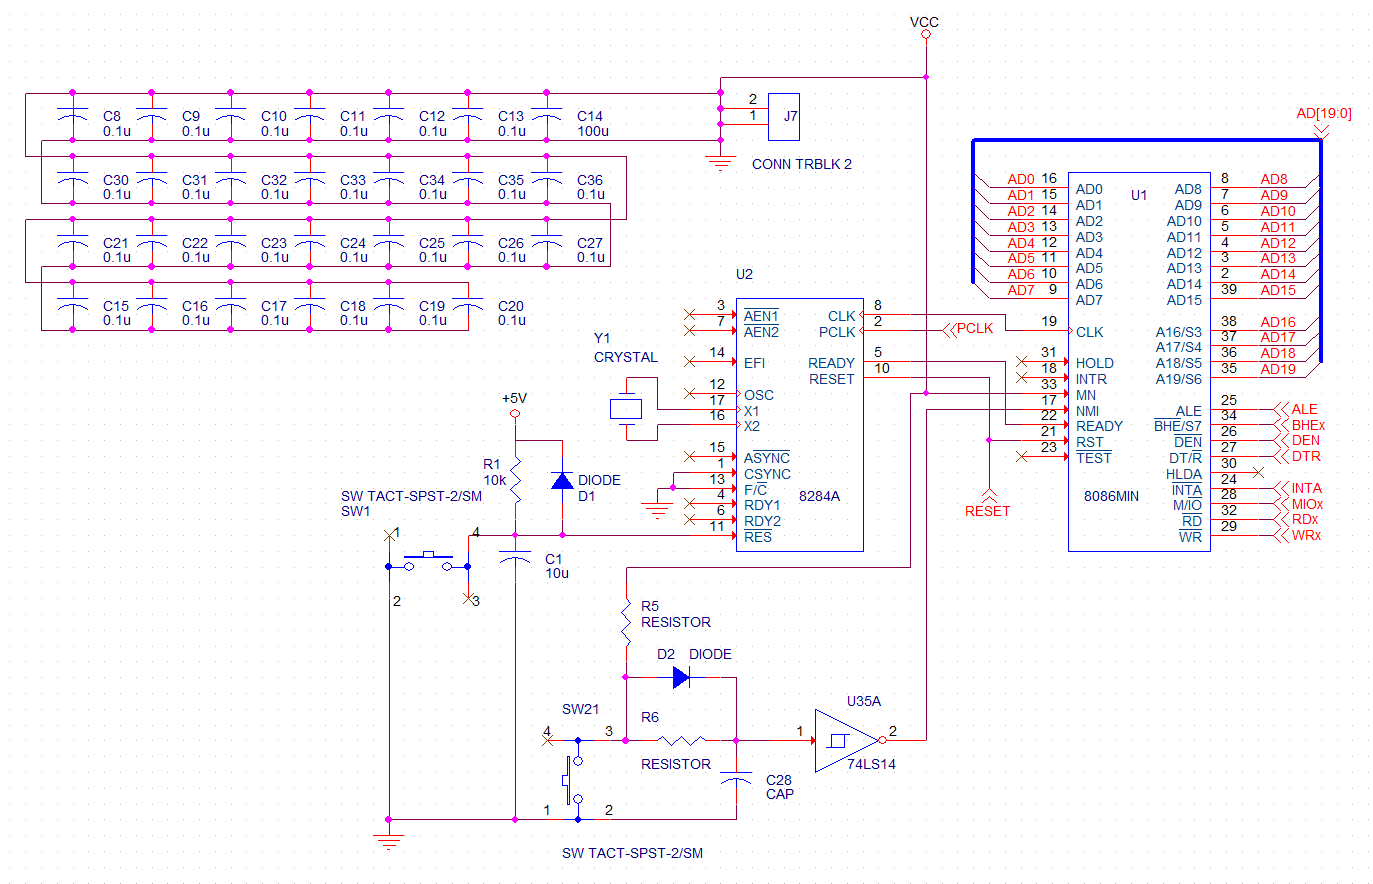
\includegraphics[width=1\textwidth]{figures/schematics/8086.png}
                \caption{8086 Interfaced with the 8284A Clock Generator and its Reset RC Push Button Circuit, and the Power Bank of the Board} \label{fig:page1}
            \end{center}
        \end{figure}

        \begin{figure}[ht]
            \begin{center}
                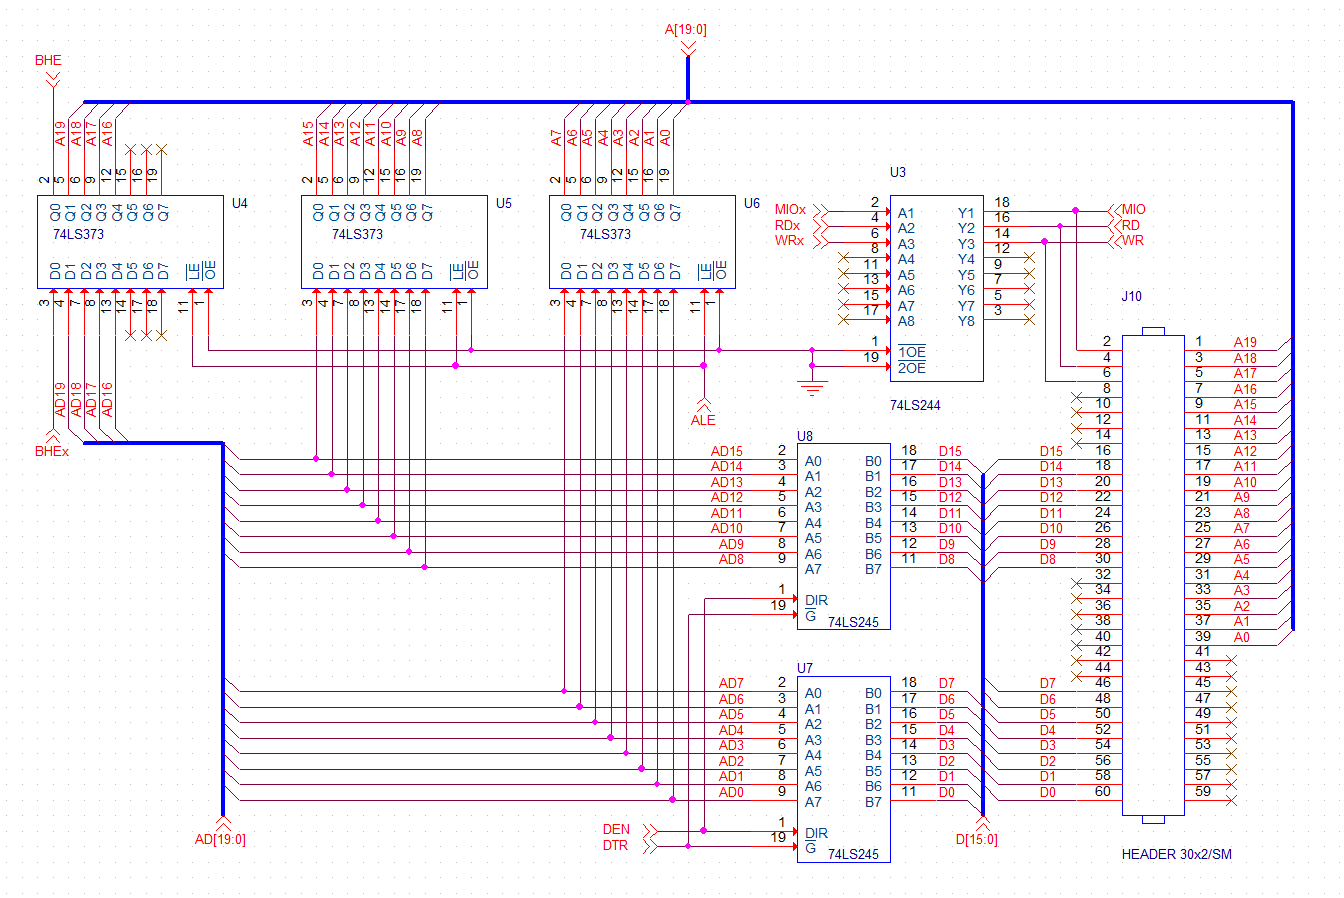
\includegraphics[width=1\textwidth]{figures/schematics/buffers.png}
                \caption{8086 Demultiplexed with Address and Data Buses Pulled into Headers} \label{fig:page2}
            \end{center}
        \end{figure}

        \begin{figure}[ht]
            \begin{center}
                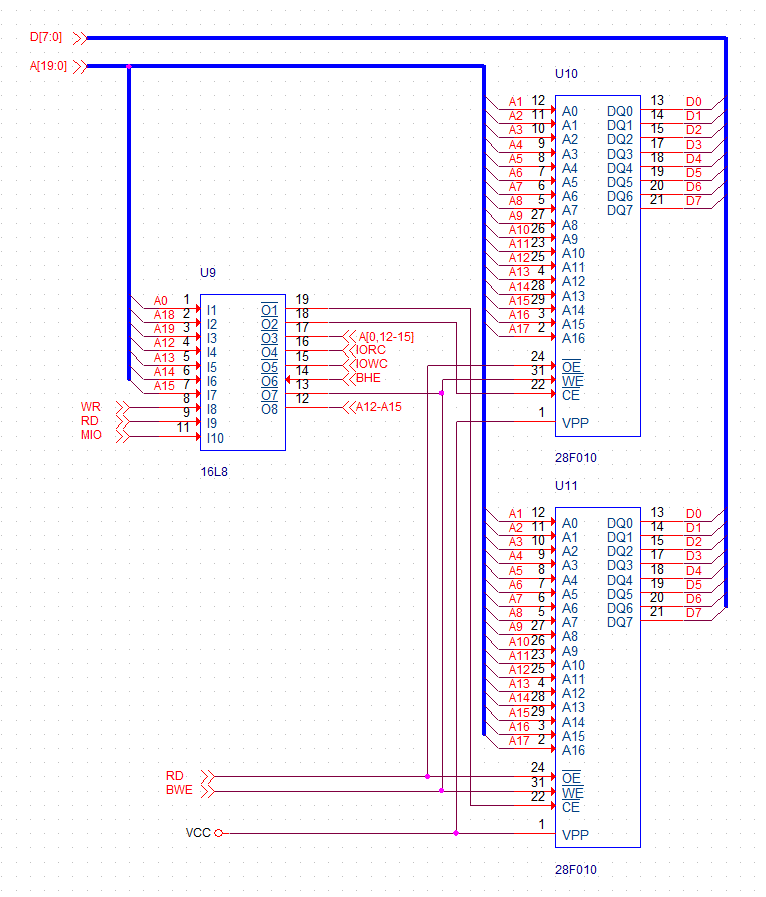
\includegraphics[width=1\textwidth]{figures/schematics/flash_mem.png}
                \caption{256 kB of CMOS Flash Memory and 128 kB Static SRAM} \label{fig:page3}
            \end{center}
        \end{figure}

        \begin{figure}[ht]
            \begin{center}
                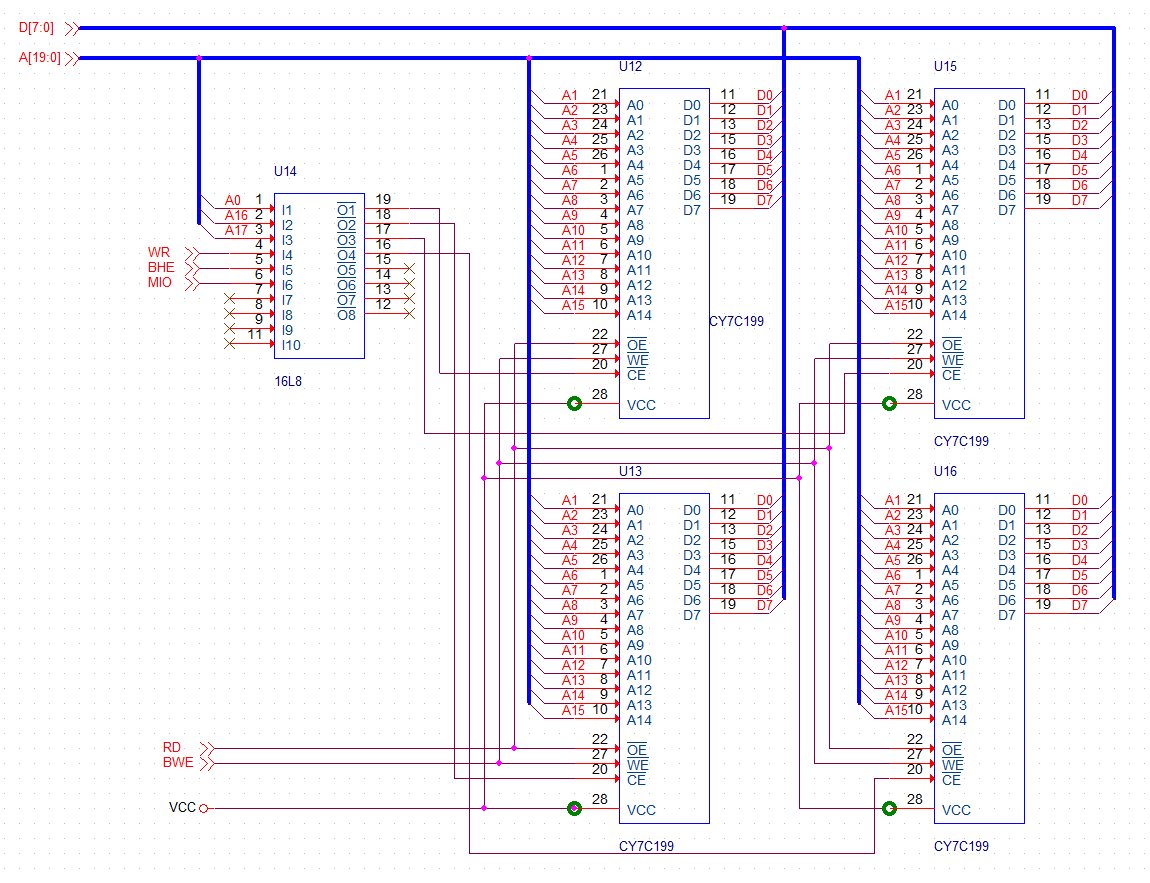
\includegraphics[width=1\textwidth]{figures/schematics/sram.png}
                \caption{128 kB Static SRAM} \label{fig:page4}
            \end{center}
        \end{figure}

        \begin{figure}[ht]
            \begin{center}
                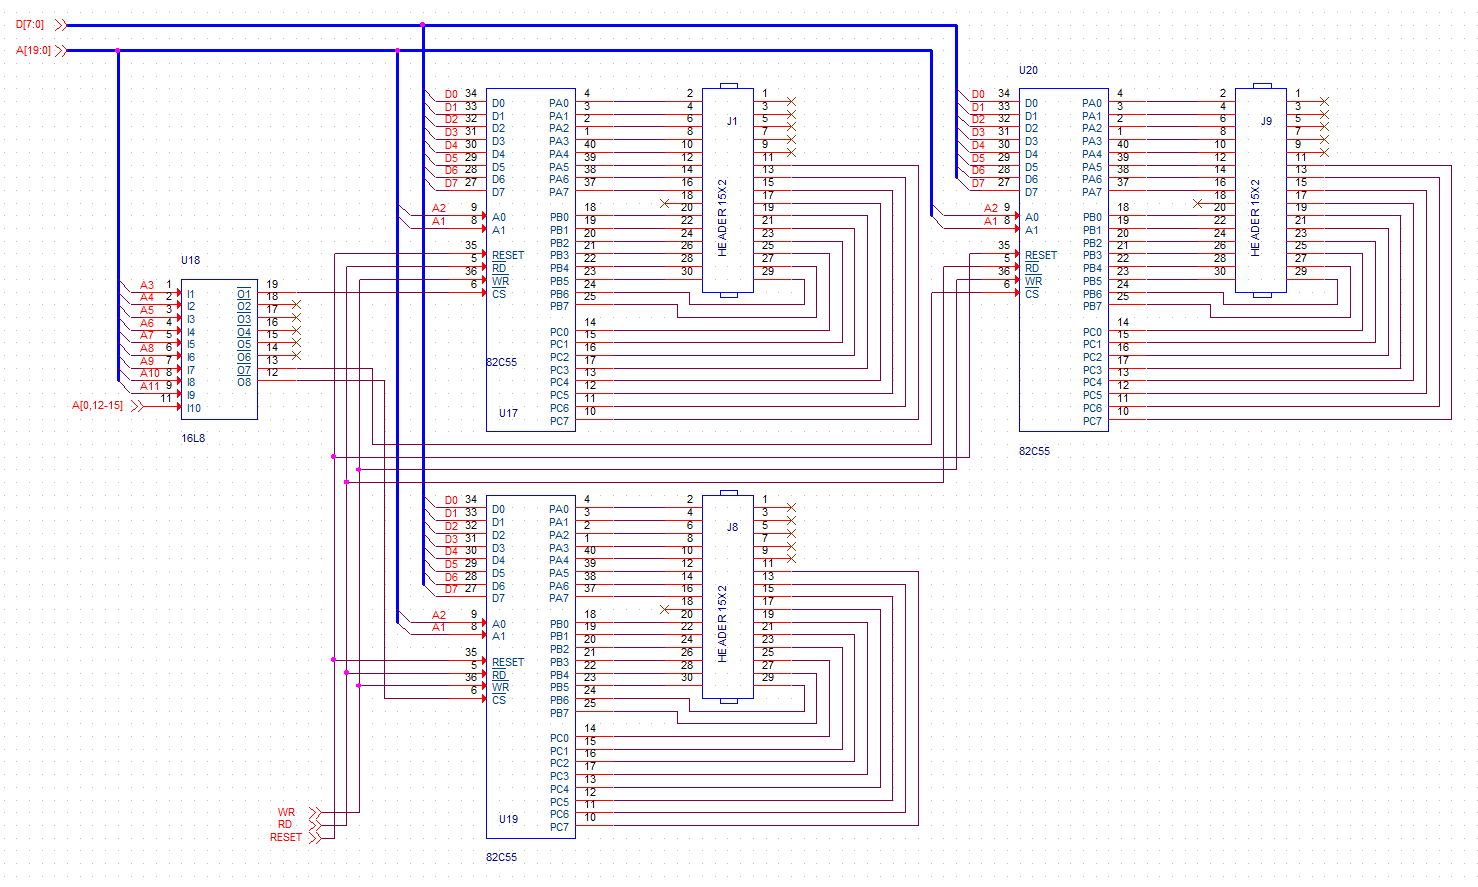
\includegraphics[width=1\textwidth]{figures/schematics/ppi.png}
                \caption{Programmable Peripheral Interface Chips with Port Connections Pulled into Headers} \label{fig:page5}
            \end{center}
        \end{figure}

        \begin{figure}[ht]
            \begin{center}
                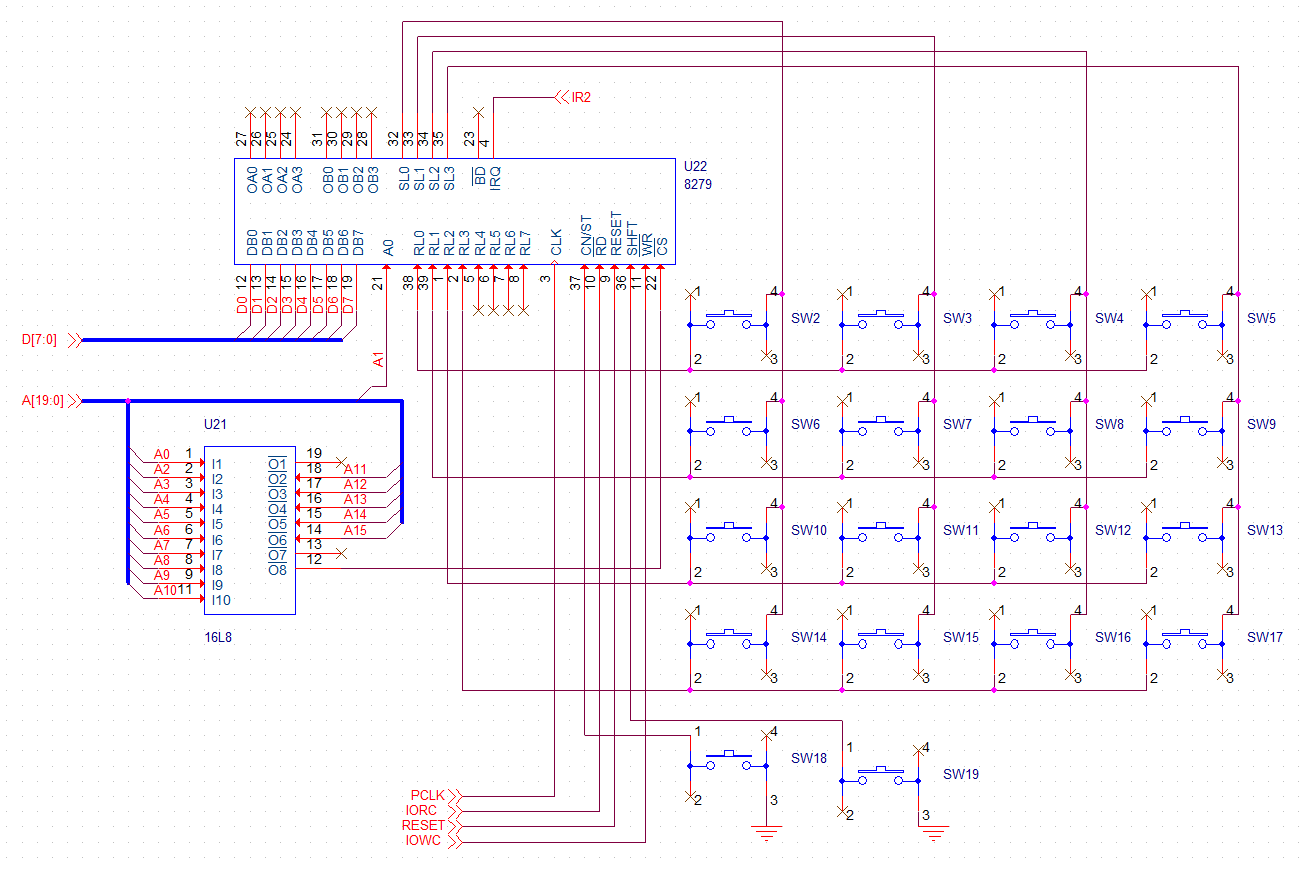
\includegraphics[width=1\textwidth]{figures/schematics/keyboard.png}
                \caption{5$\times$4 Keyboard Matrix} \label{fig:page6}
            \end{center}
        \end{figure}

        \begin{figure}[ht]
            \begin{center}
                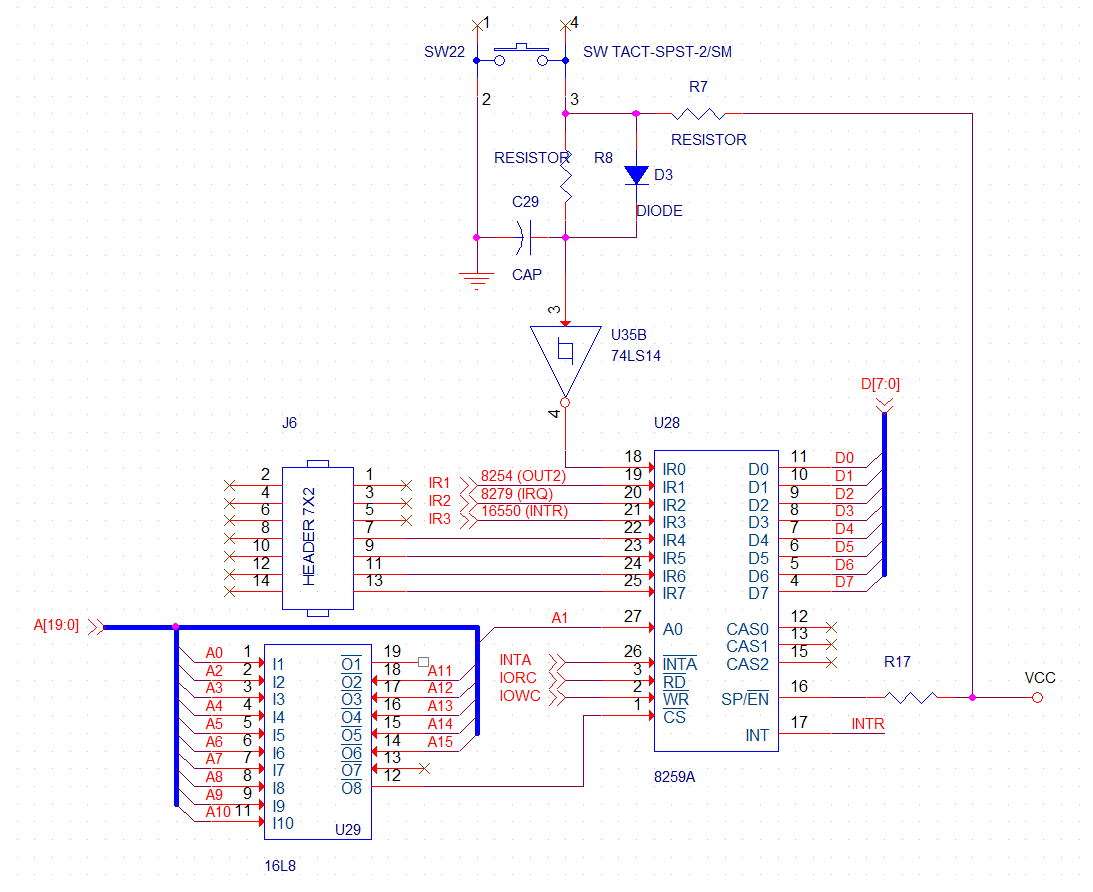
\includegraphics[width=1\textwidth]{figures/schematics/pic.png}
                \caption{Programmable Interval Timer} \label{fig:page7}
            \end{center}
        \end{figure}

        \begin{figure}[ht]
            \begin{center}
                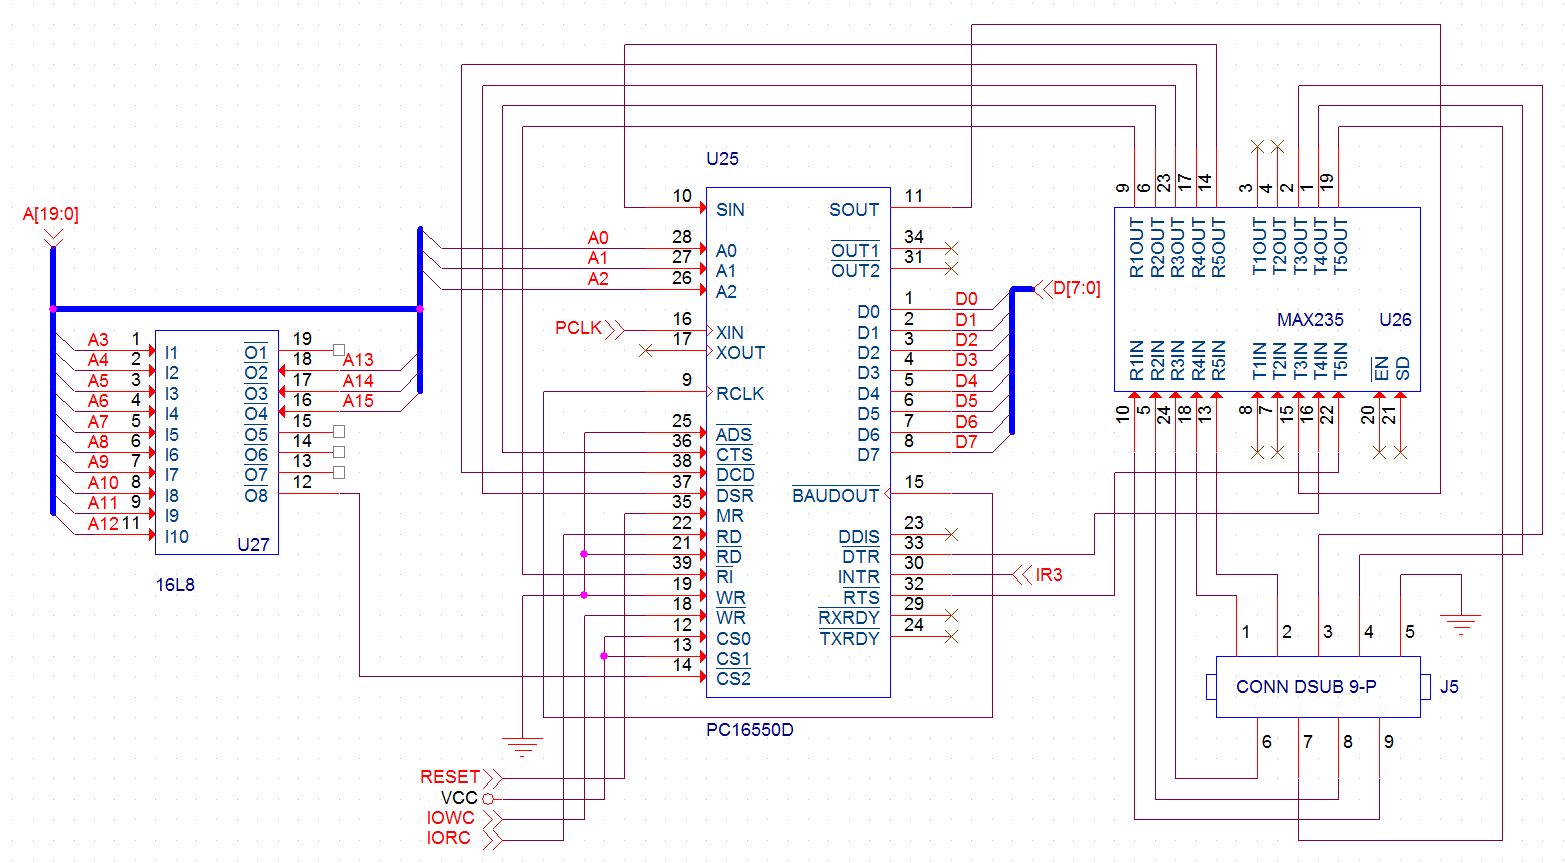
\includegraphics[width=1\textwidth]{figures/schematics/uart.png}
                \caption{UART Connected for Serial Port Using a Line Driver/Receiver and a DSUB-9 connector} \label{fig:page8}
            \end{center}
        \end{figure}

        \begin{figure}[ht]
            \begin{center}
                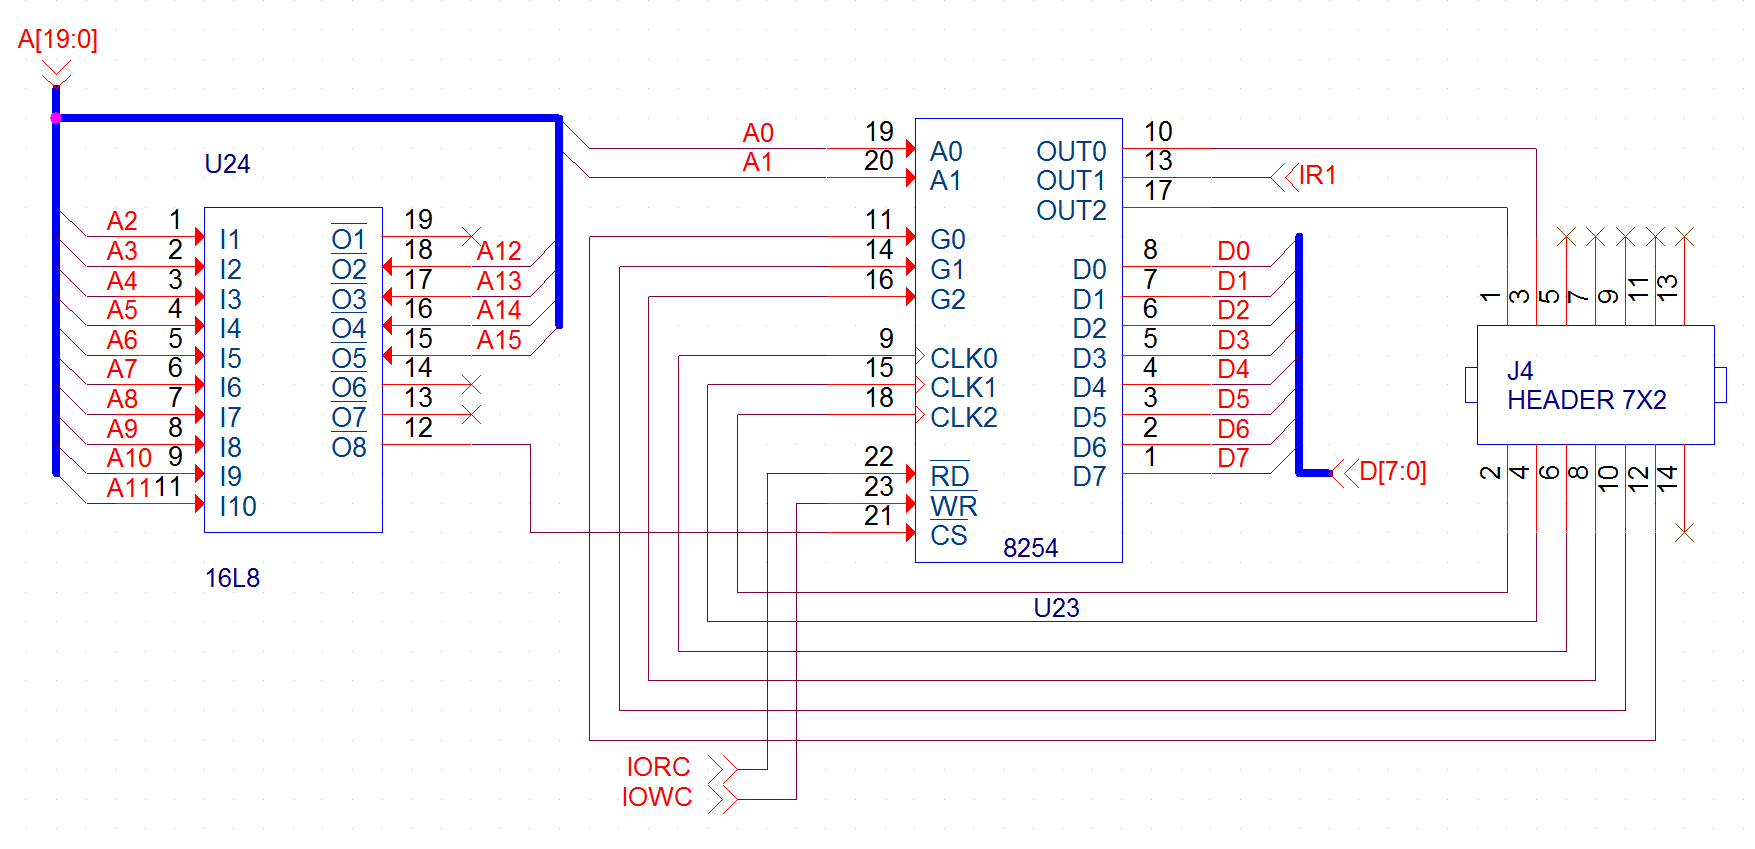
\includegraphics[width=1\textwidth]{figures/schematics/pit.png}
                \caption{Programmable Interrupt Controller with Headers for External Access} \label{fig:page9}
            \end{center}
        \end{figure}

        \begin{figure}[ht]
            \begin{center}
                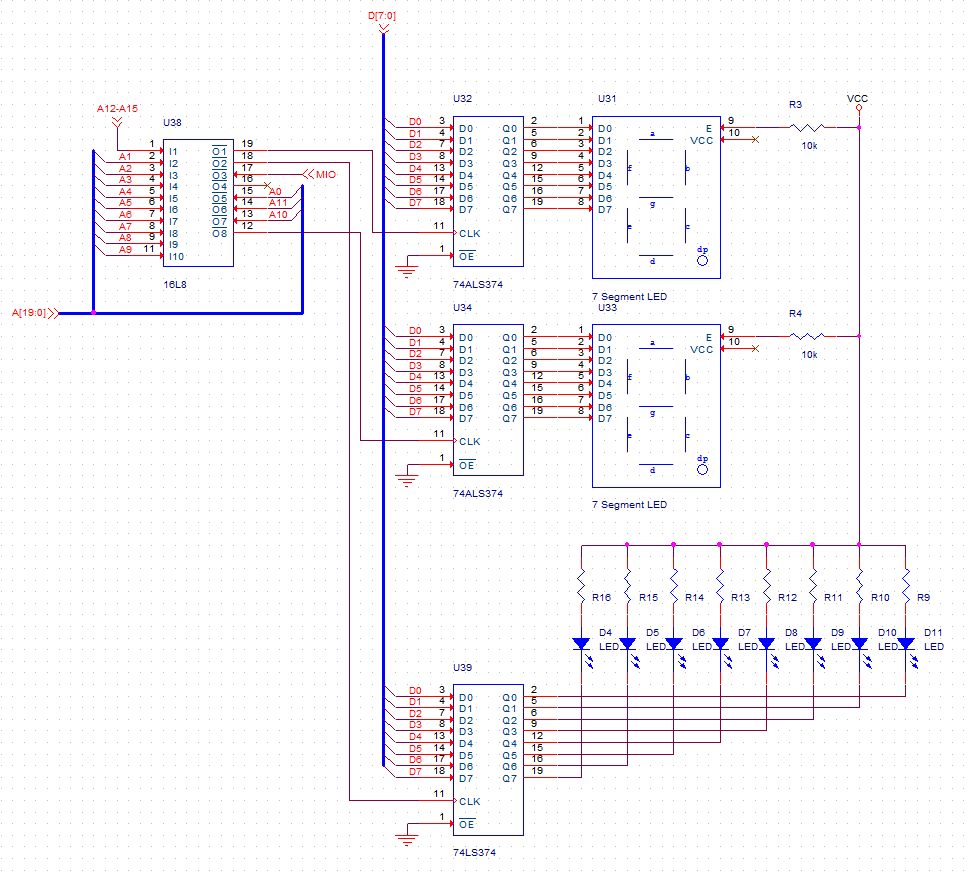
\includegraphics[width=1\textwidth]{figures/schematics/led.png}
                \caption{Common-Anode 7-Segment LEDs with 8 LEDs} \label{fig:page10}
            \end{center}
        \end{figure}

        \begin{figure}[ht]
            \begin{center}
                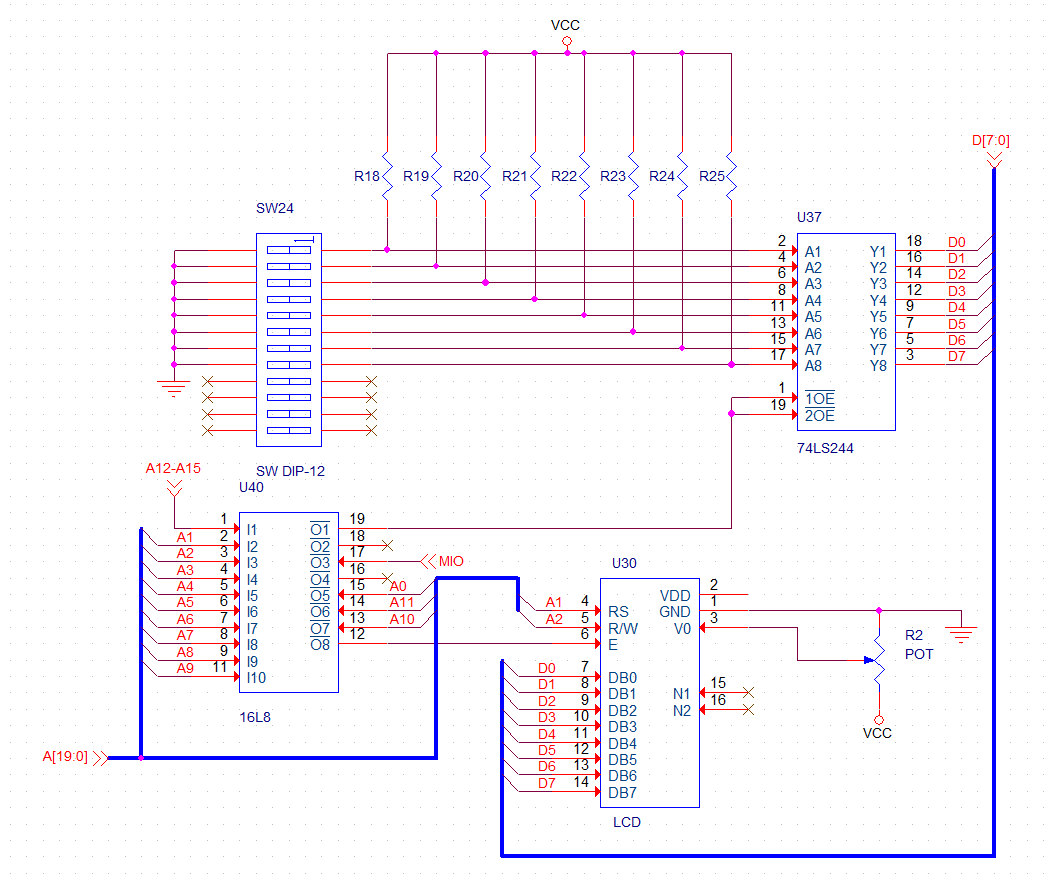
\includegraphics[width=1\textwidth]{figures/schematics/lcd.png}
                \caption{20 character $\times$ 4 line LCD Display with an Integrated LCD Controller} \label{fig:page11}
            \end{center}
        \end{figure}


    \clearpage
    \newpage

    \section{Code Implementations} \label{appendix:code}

        \subsection{Programmable Logic Devices}

            \subsubsection{U9}

                \VerbatimInput{hdl/u09.vhd}

            \newpage
            \subsubsection{U14}

                \VerbatimInput{hdl/u14.vhd}

            \newpage
            \subsubsection{U18}

                \VerbatimInput{hdl/u18.vhd}

            \newpage
            \subsubsection{U21}

                \VerbatimInput{hdl/u21.vhd}

            \newpage
            \subsubsection{U24}

                \VerbatimInput{hdl/u24.vhd}

            \newpage
            \subsubsection{U27}

                \VerbatimInput{hdl/u27.vhd}

            \newpage
            \subsubsection{U29}

                \VerbatimInput{hdl/u29.vhd}

            \newpage
            \subsubsection{U38}

                \VerbatimInput{hdl/u38.vhd}

            \newpage
            \subsubsection{U40}

                \VerbatimInput{hdl/u40.vhd}

        \newpage
        \subsection{Assembly Implementations}

            \subsubsection{LCD} \label{sec:lcd_asm}
                \VerbatimInput{assembly/lcd.asm}

            \newpage
            \subsubsection{Programmable Peripheral Interface} \label{sec:ppi_asm}
                \VerbatimInput{assembly/ppi.asm}

            \newpage
            \subsubsection{Keyboard} \label{sec:keybrd_asm}
                \VerbatimInput{assembly/keyboard.asm}

            \newpage
            \subsubsection{Programmable Interval Timer} \label{sec:pit_asm}
                \VerbatimInput{assembly/pit.asm}

            \newpage
            \subsubsection{Universal Asynchronous Receiver/Transmitter} \label{sec:uart_asm}
                \VerbatimInput{assembly/uart.asm}


    \clearpage
    \newpage

    \section{PCB Layouts} \label{appendix:pcb}

        \begin{figure}[ht]
            \begin{center}
                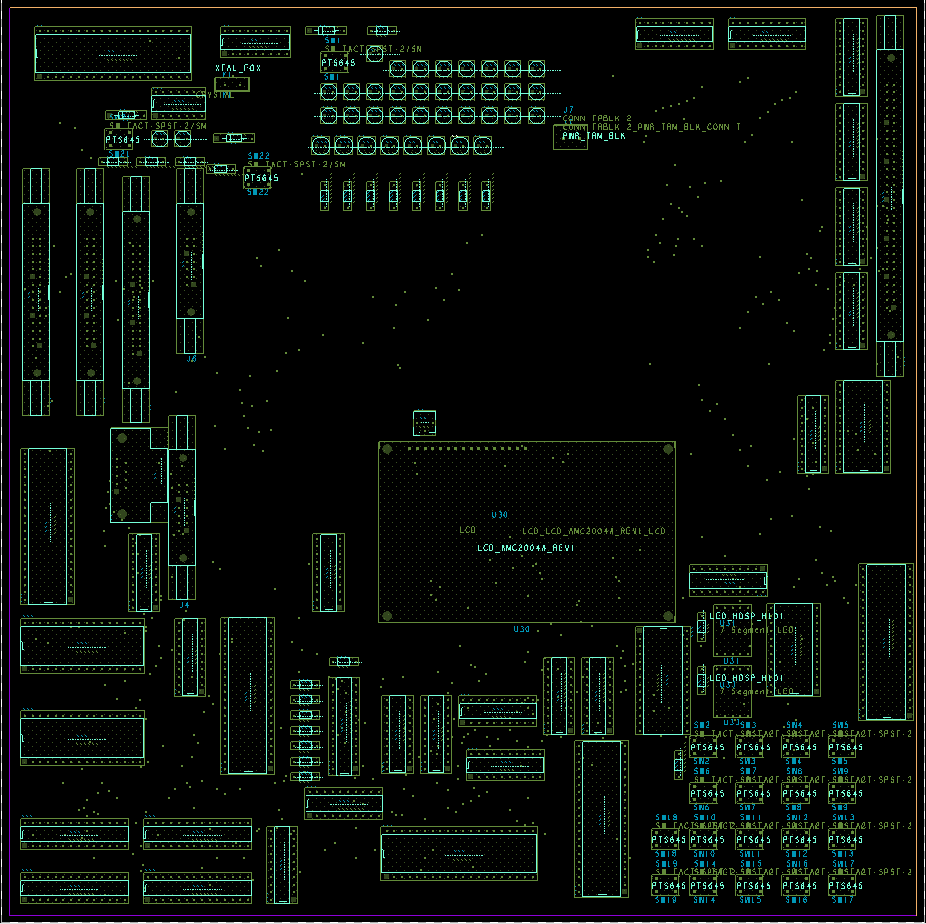
\includegraphics[width=0.9\textwidth]{figures/main.png}
                \caption{Final PCB Layout Showing Only the Components} \label{fig:main}
            \end{center}
        \end{figure}

        \begin{figure}[ht]
            \begin{center}
                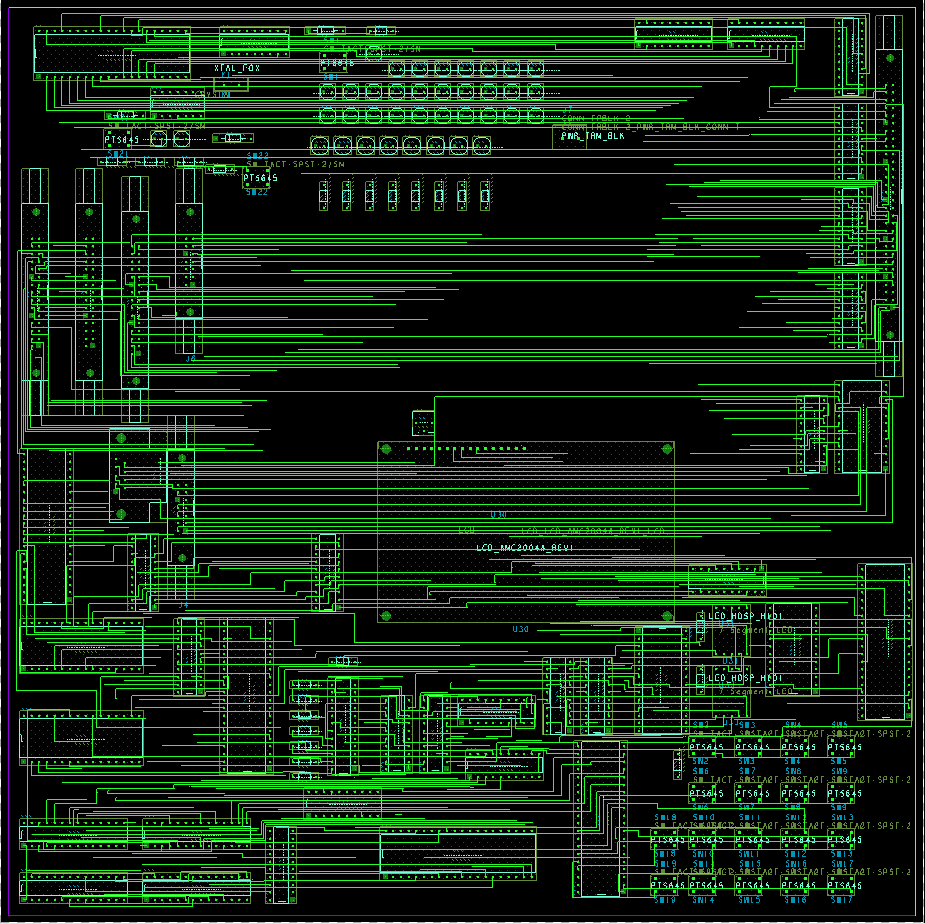
\includegraphics[width=0.95\textwidth]{figures/top.png}
                \caption{Final PCB Layout with only the Top Layer Activated} \label{fig:top}
            \end{center}
        \end{figure}

        \begin{figure}[ht]
            \begin{center}
                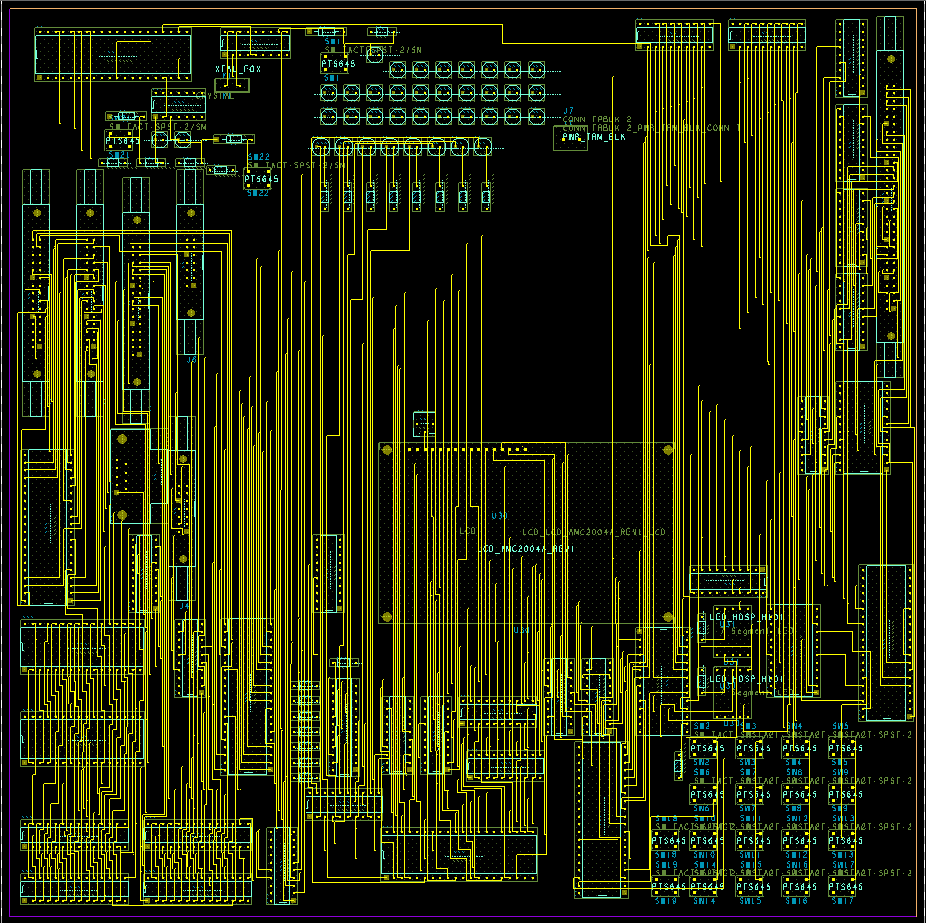
\includegraphics[width=0.95\textwidth]{figures/bottom.png}
                \caption{Final PCB Layout with only the Bottom Layer Activated} \label{fig:bottom}
            \end{center}
        \end{figure}

        \begin{figure}[ht]
            \begin{center}
                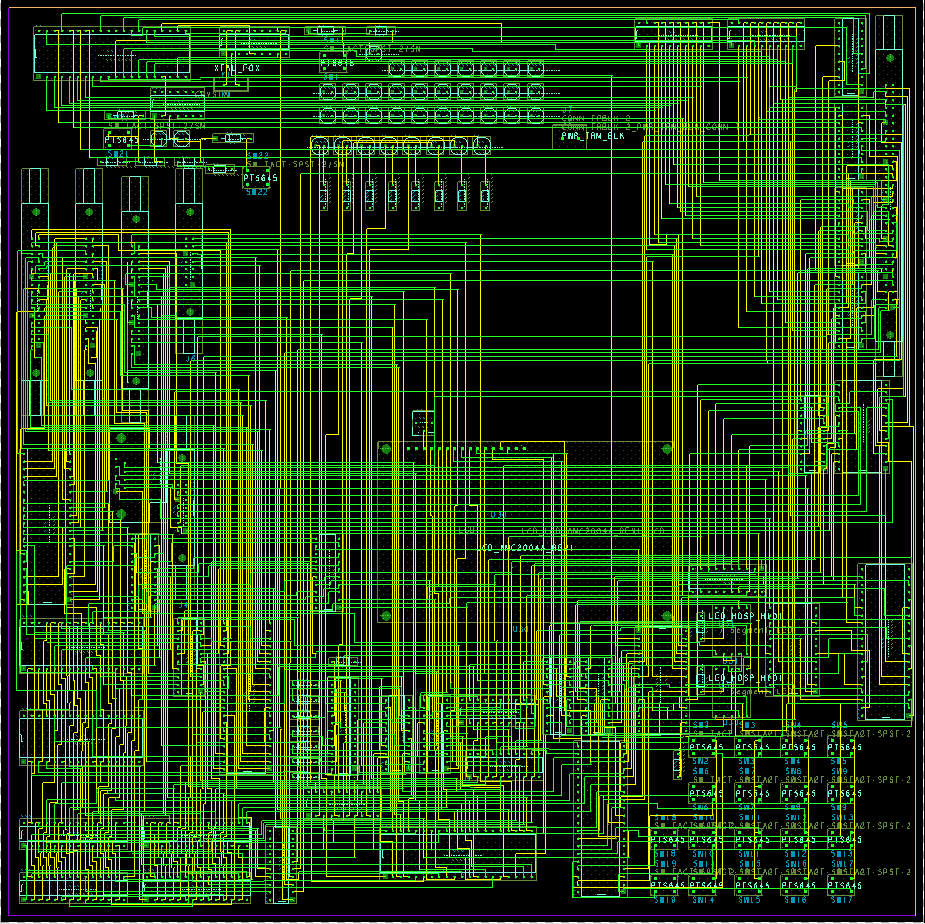
\includegraphics[width=0.95\textwidth]{figures/board.png}
                \caption{Final PCB Layout with all Layers Activated} \label{fig:board}
            \end{center}
        \end{figure}

        \begin{figure}[ht]
            \begin{center}
                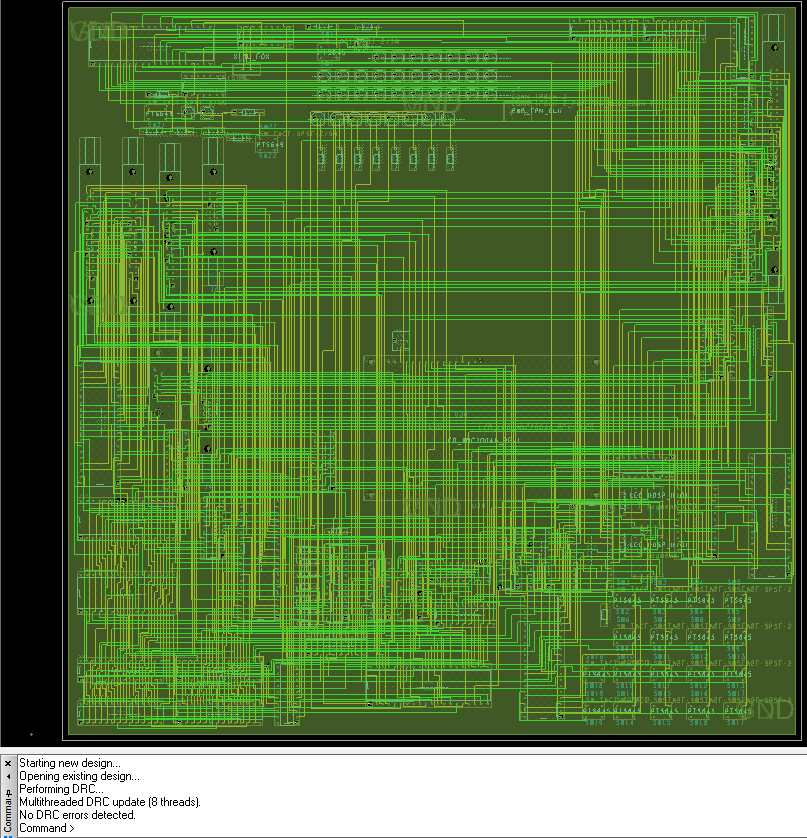
\includegraphics[width=0.95\textwidth]{figures/all.png}
                \caption{Final PCB Layout with all Layers Activated, including Power and Ground} \label{fig:all}
            \end{center}
        \end{figure}

        \clearpage
        \newpage

    \section{Bill of Materials} \label{appendix:bom}

        \def\arraystretch{1.22}
        \begin{table}[H]
            \footnotesize
            \begin{tabular*}{100pt}{@{\extracolsep{\fill}} c p{10cm} p{10cm}}
                \textbf{Amount} & \textbf{Part} & \textbf{Description} \\
                1 & C1 & 10u \\
                26 & C8,C9,C10,C11,C12,C13,C15,C16,\newline
                C17,C18,C19,C20,C21,C22,C23,C24,C25,\newline 
                C26,C27,C30,C31,C32,C33,C34,C35,C36 & 0.1u \\
                1 & C14 & 100u \\
                2 & C28,C29 & CAP \\
                3 & D1,D2,D3 & DIODE \\
                8 & D4,D5,D6,D7,D8,D9,D10,D11 & LED \\
                3 & J1,J8,J9 & HEADER 15X2 \\
                2 & J4,J6 & HEADER 7X2 \\
                1 & J5 & CONN DSUB 9-P \\
                1 & J7 & CONN TRBLK 2 \\
                1 & J10 & HEADER 30x2/SM \\
                11 & R1,R3,R4,R18,R19,R20,R21,R22,\newline
                R23,R24,R25 & 10k \\
                1 & R2 & POT \\
                13 & R5,R6,R7,R8,R9,R10,R11,R12,R13,\newline
                R14,R15,R16,R17 & RESISTOR \\
                3 & SW1,SW21,SW22 & SW TACT-SPST-2/SM \\
                18 & SW2,SW3,SW4,SW5,SW6,SW7,SW8,SW9,\newline
                SW10,SW11,SW12,SW13,SW14,SW15,SW16,SW17,\newline
                SW18,SW19 & SW TACT-SPST-2 \\
                1 & SW24 & SW DIP-12 \\
                1 & U1 & 8086MIN \\
                1 & U2 & 8284A \\
                2 & U3,U37 & 74LS244 \\
                3 & U4,U5,U6 & 74LS373 \\
                2 & U7,U8 & 74LS245 \\
                9 & U9,U14,U18,U21,U24,U27,U29,U38,U40 & 16L8 \\
                2 & U10,U11 & 28F010 \\
                4 & U12,U13,U15,U16 & CY7C199 \\
                3 & U17,U19,U20 & 82C55 \\
                1 & U22 & 8279 \\
                1 & U23 & 8254 \\
                1 & U25 & PC16550D \\
                1 & U26 & MAX235 \\
                1 & U28 & 8259A \\
                1 & U30 & LCD \\
                2 & U31,U33 & 7 Segment LED \\
                2 & U32,U34 & 74ALS374 \\
                1 & U35 & 74LS14 \\
                1 & U39 & 74LS374 \\
                1 & Y1 & CRYSTAL \\
            \end{tabular*}
        \end{table}

        \clearpage

\end{appendices}
    \newpage
\addcontentsline{toc}{section}{References}
    \begin{thebibliography}{9}

    \bibitem{buses} DBHJDS\\
    http://gradestack.com/Microprocessors-and/Architecture-of-8086-and/Address-Bus-Data-Bus-/19317-3912-38171-study-wtw

    \bibitem{pal} Programmable Array Logic\\
    https://www.electrical4u.com/programmable-array-logic/

    \end{thebibliography}


\end{document}
